\documentclass[12pt,a4paper,titlepage]{article}
\usepackage[utf8]{inputenc} % para poder colocar acentos e caracteres especiais
\usepackage[portuguese]{babel}
\usepackage{graphicx} % Permite inserir e manipular imagens
\usepackage{fancyhdr} 
\usepackage{geometry} % Permite definir facilmente margens e o layout da página
\usepackage{setspace} % Permite alterar o espaçamento entre linhas
\usepackage{titlesec} % Permite personalizar os títulos de secções e subseções
\usepackage[hidelinks]{hyperref} % Ativa links clicáveis no PDF
\usepackage{multicol} % coloca isto no preâmbulo

% Configuração do listings (paraexcertos de código)
\usepackage{listings}
\usepackage{xcolor}

\usepackage{caption}
\usepackage{subcaption}

\definecolor{codegreen}{rgb}{0,0.6,0}
\definecolor{codegray}{rgb}{0.5,0.5,0.5}
\definecolor{codepurple}{rgb}{0.58,0,0.82}
\definecolor{backcolour}{rgb}{0.95,0.95,0.92}
\renewcommand{\lstlistingname}{Excerto} % Colocar como excerto no pdf e não como Listing
\lstdefinestyle{mystyle}{
	backgroundcolor=\color{backcolour},   
	commentstyle=\color{codegreen},
	keywordstyle=\color{magenta},
	numberstyle=\tiny\color{codegray},
	stringstyle=\color{codepurple},
	basicstyle=\ttfamily\footnotesize,
	breakatwhitespace=false,         
	breaklines=true,                 
	captionpos=b,                    
	keepspaces=true,                 
	numbers=left,                    
	numbersep=5pt,                  
	showspaces=false,                
	showstringspaces=false,
	showtabs=false,                  
	tabsize=2
}
\lstset{style=mystyle}
% Ensinar o listings UTF-8
\lstset{
	extendedchars=true,
	literate=
	{á}{{\'a}}1 {é}{{\'e}}1 {í}{{\'i}}1 {ó}{{\'o}}1 {ú}{{\'u}}1
	{Á}{{\'A}}1 {É}{{\'E}}1 {Í}{{\'I}}1 {Ó}{{\'O}}1 {Ú}{{\'U}}1
	{à}{{\`a}}1 {è}{{\`e}}1 {ì}{{\`i}}1 {ò}{{\`o}}1 {ù}{{\`u}}1
	{À}{{\`A}}1 {È}{{\'E}}1 {Ì}{{\`I}}1 {Ò}{{\`O}}1 {Ù}{{\`U}}1
	{â}{{\^a}}1 {ê}{{\^e}}1 {î}{{\^i}}1 {ô}{{\^o}}1 {û}{{\^u}}1
	{Â}{{\^A}}1 {Ê}{{\^E}}1 {Î}{{\^I}}1 {Ô}{{\^O}}1 {Û}{{\^U}}1
	{ã}{{\~a}}1 {õ}{{\~o}}1 {Ã}{{\~A}}1 {Õ}{{\~O}}1
	{ç}{{\c c}}1 {Ç}{{\c C}}1
}

% Page setup
\geometry{margin=2.5cm}
\setstretch{1.5}
\pagestyle{fancy}
\fancyhf{}
\rhead{\thepage}
\lhead{Escola Superior de Tecnologia e Gestão}

% Title formatting
\titleformat{\section}{\large\bfseries}{\thesection}{1em}{}
\titleformat{\subsection}{\normalsize\bfseries}{\thesubsection}{1em}{}

\begin{document}

% Title Page
\begin{titlepage}
    \centering
    
\includegraphics[width=15cm]{imagens/estg_logo.png}\par\vspace{0.9cm} % 
    \scshape % Small caps for the institution name
    
    \rule{\textwidth}{1pt}\vspace{0.4cm} % Horizontal line
    {\Huge \bfseries Monitorização de Sensores IoT \par}
    {Paradigmas Emergentes para o Desenvolvimento Web e Mobile\par}
    \vspace{0.4cm}\rule{\textwidth}{1pt}\par
    \vspace{2cm}
    
    \Large Mestrado em Engenharia Informática \par
    \vspace{4cm}

    \normalsize
    \textbf{Grupo 1} \par
    Diogo Pereira – 8200594 \par
    Hugo Guimarães – 8220337 \par
    \vfill

    \large \today
\end{titlepage}


% Indice
\tableofcontents
\newpage

% Lista de Figuras
\renewcommand{\listfigurename}{Índice de Figuras}
\listoffigures
\newpage

% Lista de Tabelas
%\renewcommand{\listtablename}{Índice de Tabelas}
%\listoftables
%\addcontentsline{toc}{section}{Índice de Tabelas}
%\newpage

\renewcommand{\lstlistlistingname}{Índice de Excertos de Código}
\lstlistoflistings



\section{Introdução} \label{sec:introducao}

\subsection{Contextualização e Tema do Projeto}

No cenário tecnológico atual, o quotidiano das pessoas e das organizações é cada vez mais rodeado por redes de dispositivos inteligentes e sensores que recolhem dados em tempo real. Estes sensores, que podem medir variáveis como a qualidade do ar, temperatura e humidade, geram fluxos contínuos de informação que exigem sistemas robustos capazes de os processar e transformar em conhecimento útil. 

Foi com base nesta necessidade que o presente projeto foi desenvolvido, assumindo-se como um elemento integrador no âmbito da unidade curricular de Paradigmas Emergentes para o Desenvolvimento Web e Mobile do Mestrado em Engenharia Informática. O trabalho propõe o desenvolvimento de uma aplicação para a gestão e monitorização de uma rede de sensores IoT (Internet of Things) simulados. Para dar resposta a este desafio e garantir uma arquitetura resiliente e reativa, a solução foi desenhada com base em três pilares fundamentais exigidos: Programação Funcional, Programação Orientada a Aspetos e Programação \textit{Event-Driven} (Orientada a Eventos). O sistema permite a monitorização contínua destes dados em tempo real através de plataformas Web e Mobile.

\subsection{Objetivos do Trabalho}

Este trabalho prático tem como principal objetivo consolidar e integrar os conhecimentos adquiridos durante a unidade curricular, estimulando a exploração de conceitos avançados e tecnologias emergentes. 

Para a concretização deste propósito principal, foram definidos os seguintes objetivos específicos:
\begin{itemize}
	\item \textbf{Aplicação de Paradigmas Emergentes:} Desenvolver a arquitetura do sistema aplicando os conceitos de Programação Funcional (garantindo imutabilidade e funções puras), Programação Orientada a Aspetos (separando preocupações transversais como \textit{logs} ou métricas) e Programação \textit{Event-Driven} (para lidar com o fluxo de dados dos sensores).
	\item \textbf{Desenvolvimento Multiplataforma:} Construir a solução contendo, no mínimo, um componente \textit{front-end} para \textit{Web} e outro para ambiente \textit{Mobile}, garantindo a acessibilidade aos \textit{dashboards} de monitorização.
	\item \textbf{Comunicação em Tempo Real e Eficiente:} Utilizar \textit{WebSockets} para o envio de eventos e alertas instantâneos para os clientes, e integrar \textit{GraphQL} para otimizar as consultas de dados, evitando \textit{over-fetching}.
	\item \textbf{Gestão de Dispositivos IoT:} Capacitar a aplicação para gerir múltiplos sensores em simultâneo, processar as suas leituras e fornecer alertas em tempo real perante anomalias (e.g., aumentos súbitos de temperatura).
\end{itemize}

\subsection{Estrutura do Relatório}

O presente relatório está organizado de forma a detalhar todo o processo de conceção e desenvolvimento da solução. A Secção \ref{sec:Tecnologias_Utilizadas} apresenta as tecnologias escolhidas para o \textit{front-end} e \textit{back-end}. A Secção \ref{sec:arquitetura_solucao} expõe a arquitetura da solução, acompanhada do respetivo diagrama arquitetural e dos diagramas UML necessários para o seu entendimento técnico. A Secção \ref{sec:paradigmas_implementacao} detalha o mapeamento dos objetivos com o trabalho desenvolvido, nomeadamente a forma como os paradigmas Funcional, Orientado a Aspetos e \textit{Event-Driven} foram implementados no código. A Secção \ref{sec:demonstracao} foca-se na demonstração das interfaces concebidas (Web e Mobile) e na exploração das suas funcionalidades. A Secção \ref{sec:desempenho_individual} apresenta um gráfico detalhado com os \textit{story points} atribuídos e concluídos ao longo do projeto, evidenciando o desempenho e esforço individual de cada estudante. Por fim, a Secção \ref{sec:conclusao} realiza uma breve súmula do trabalho, enumerando as conclusões retiradas e possíveis linhas de trabalho futuro.

\section{Tecnologias Utilizadas} \label{sec:Tecnologias_Utilizadas}

\subsection{Flutter (Front-end Web e Mobile)}

O motivo por detrás da escolha do Flutter para a realização deste projeto reside na flexibilidade do mesmo de poder ser facilmente compilado para diversas plataformas. A solução foi estruturada em duas aplicações: um \textit{dashboard Web} e aplicação \textit{Mobile}. Para evitar a duplicação de esforço e garantir a consistência, ambas as partes estão unidas por um \textit{package} interno partilhado, que centraliza as entidades, a gestão de estado e toda a lógal com o \textit{back-end}.

Outro dos motivos para a escolha desta tecnologia foi a alta performance para renderizar o conteúdo no ecrã. Ao desenhar cada pixel diretamente no ecrã de forma independente do sistema operativo, o Flutter permite que gráficos de monitorização dos sensores e sejam executados de forma fluida, tanto num navegador \textit{Web} como num dispositivo \textit{Mobile} com recursos mais limitados.

\subsection{Scala e ZIO (Back-end)}
O Scala em conjunto com o ecossistema ZIO foi adotado de modo a cumprir os requisitos arquiteturais impostos para este projeto, nomeadamente a aplicação dos três paradigmas emergentes. 
Em primeiro lugar, a linguagem Scala fomenta nativamente a programação funcional, garantindo que a validação e transformação dos dados dos sensores é feita através de funções puras e estruturas de dados imutáveis, eliminando efeitos secundários indesejados. 

% TODO validar se usei ZStreams
Em segundo lugar, a biblioteca ZIO oferece abstrações como as \textit{ZStreams}, que foram essenciais para implementar a programação orientada a eventos. Em vez de um modelo de pedido-resposta tradicional, o sistema processa um fluxo contínuo de leituras (\textit{pipeline} de eventos) proveniente dos sensores, filtrando anomalias e publicando alertas de forma reativa.

% TODO validar se isto é verdade
Por fim, o ZIO suporta nativamente a programação orientada a aspetos através de \textit{ZIO Aspects}. Isto permitiu isolar preocupações transversais, como o registo de \textit{logs} de todas as leituras e medição de métricas de latência. Assim, o código permanece limpo e focado apenas no processamento da telemetria, enquanto os aspetos são aplicados de forma declarativa e invisível. A alta concorrência é garantida através das \textit{Fibers} do ZIO, que, à semelhança das \textit{Goroutines}, são bastante leves e permitem ao servidor suportar milhares de eventos concorrentes com um consumo mínimo de memória.

\subsection{C++ (Simulação de Sensores IoT)}
Embora os sensores deste projeto sejam simulados, a escolha da linguagem C++ foi deliberada para manter a máxima fidelidade com os ambientes de Internet of Things (IoT) do mundo real. Na indústria, a maior parte dos microcontroladores (como o ecossistema Arduino ou o ESP32) é programada em C ou C++ devido ao controlo de baixo nível sobre a memória e o \textit{hardware}. 

Ao desenvolver os simuladores em C++, o projeto mimetiza o comportamento, as restrições e o formato de dados que um sensor de temperatura, humidade ou qualidade do ar real emitiria. Estes simuladores atuam como os produtores iniciais no fluxo de dados, gerando eventos a uma taxa configurável que alimentam o \textit{broker} de mensagens e, consequentemente, todo o \textit{pipeline} reativo do \textit{back-end}.


\section{Arquitetura da Solução} \label{sec:arquitetura_solucao}

O sistema está representado na Figura \ref{fig:arquitetura}, encontra-se dividido em três camadas: Simulador, \textit{Back-end} e \textit{Front-end}. O fluxo de informação ocorre de forma descendente no que toca à telemetria, e de forma bidirecional na interação com o cliente.

\begin{figure}[htb]
	\centering
	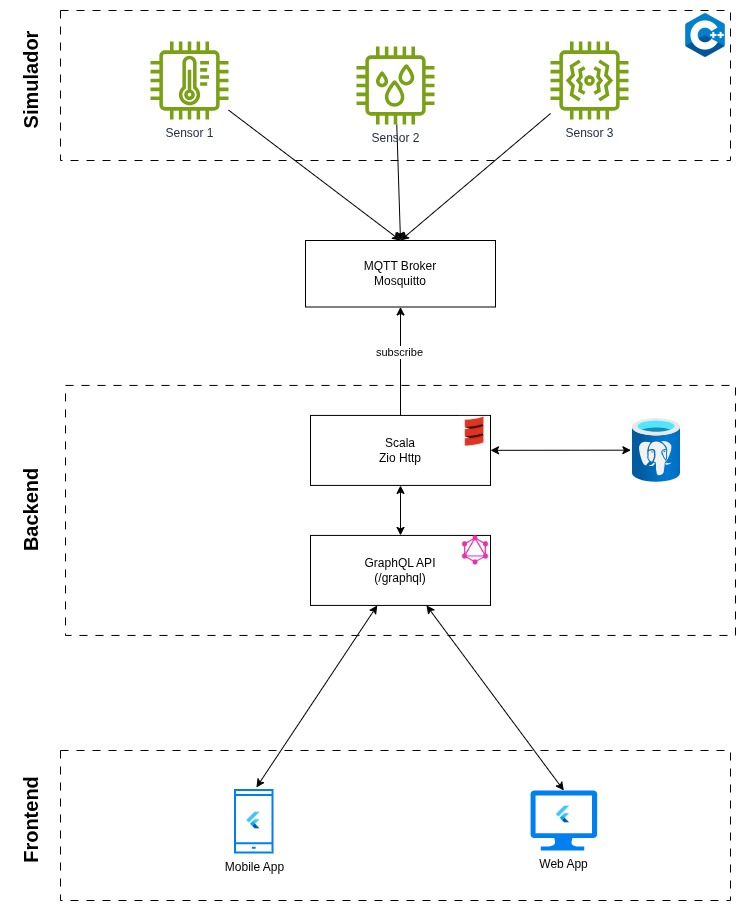
\includegraphics[width=0.6\textwidth]{imagens/architeture.jpg}
	\caption{Diagrama de Arquitetura de Alto Nível}
	\label{fig:arquitetura}
\end{figure}


\subsection{Camada de Simulação (Ingestão de Dados)}
Na camada superior encontram-se os componentes desenvolvidos em C++, responsáveis por mimetizar o comportamento de dispositivos físicos num ambiente IoT (Sensores 1, 2 e 3). Estes simuladores geram medições contínuas (como temperatura e humidade) e atuam como produtores (\textit{publishers}). Os dados gerados são enviados para um \textit{Broker} MQTT (neste caso, o \textit{Mosquitto}) seguindo a especificação Sparkplug B. Esta convenção tira partido de \textit{Protocol Buffers} (Protobuf) para a serialização binária dos dados, um padrão que reduz drasticamente o tamanho do \textit{payload} e acelera a comunicação. A escolha do MQTT e do Sparkplug B justifica-se por constituir o ecossistema padrão e mais eficiente na comunicação \textit{machine-to-machine} (M2M) na indústria.

\subsection{\textit{Back-end} (Processamento e Persistência)}
O Back-end, desenvolvido em Scala com recurso à biblioteca \textit{ZIO} e \textit{ZIO HTTP}. O fluxo de operações decorre da seguinte forma:
\begin{itemize}
	\item \textbf{Subscrição e Processamento:} O servidor Scala atua como cliente do \textit{broker} MQTT, subscrevendo os tópicos dos sensores. À medida que as mensagens chegam, entram numa \textit{pipeline}, onde a informação é validada e filtrada. % TODO ainda não sei se tenho validação (deve entrar tudo)
	\item \textbf{Armazenamento de Histórico:} O \textit{back-end} comunica com uma base de dados relacional PostgreSQL para persistir os dados processados.
	\item \textbf{Interface de Comunicação:} Para servir as aplicações cliente, o servidor expõe uma API GraphQL.
\end{itemize}

\subsection{\textit{Front-end} (Visualização Web e Mobile)}
Na camada de \textit{Front-end} encontram-se a aplicação para dispositivos móveis e a aplicação \textit{Web}, ambas desenvolvidas na \textit{framework} Flutter a partir de um \textit{package} partilhado entre as duas, evitando duplicação desnecessária de código. 

Estas aplicações comunicam exclusivamente com o serviço de \textit{Back-end} através da API GraphQL. Esta ligação reflete-se na arquitetura através das setas bidirecionais, pois o cliente não realiza apenas \textit{Queries} (pedidos HTTP) para obter o histórico guardado no PostgreSQL. Crucialmente, as aplicações cliente estabelecem ligações persistentes via \textit{WebSockets} (através de \textit{Subscriptions} GraphQL) com o servidor Scala. Isto garante que sempre que um novo evento passa pela \textit{pipeline} do \textit{back-end}, os \textit{dashboards} Flutter são atualizados em tempo real, sem necessidade de \textit{polling} constante.

% TODO validar mais tarde se isto está correto
\subsection{Fluxo de Dados e Interação}
Todo o fluxo de dados da aplicação está descrito na Figura \ref{fig:sequencia}, que demonstra o comportamento dinâmico e a interação em tempo real entre as três camadas descritas anteriormente.

\begin{figure}[htb]
	\centering
	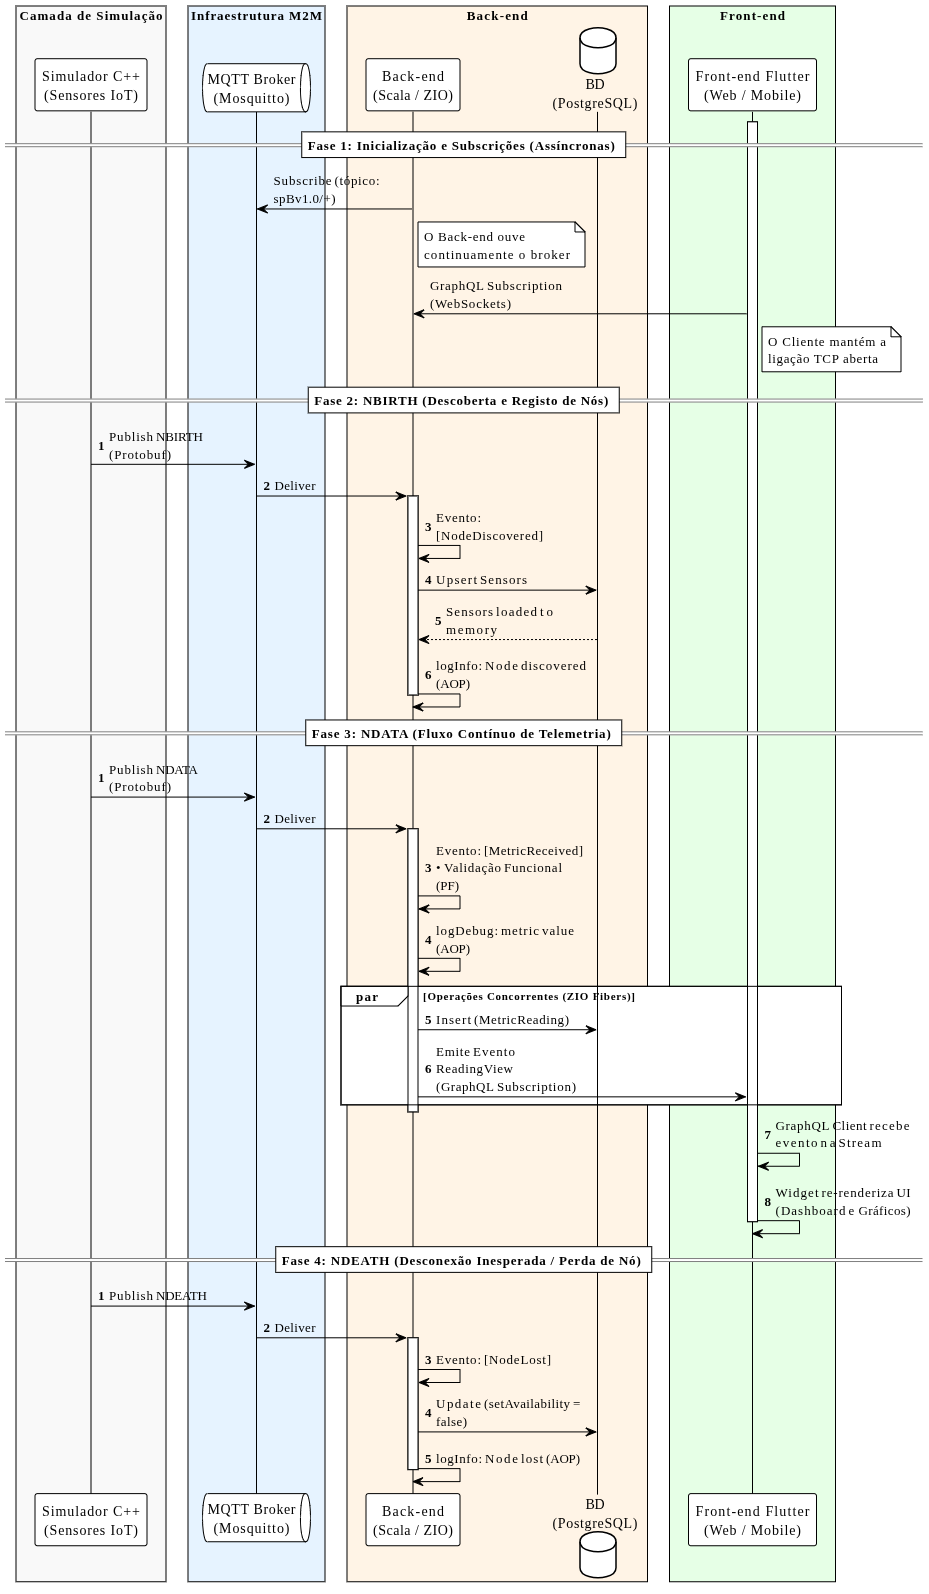
\includegraphics[width=0.8\textwidth]{imagens/messages_sequence_diagram.png}
	\caption{Diagrama de Sequência ilustrando o fluxo de eventos em tempo real.}
	\label{fig:sequencia}
\end{figure}

O processo inicia-se de forma assíncrona, com o servidor Scala e a aplicação Flutter a estabelecerem as respetivas subscrições. A partir desse momento, o sistema entra num ciclo contínuo onde a telemetria publicada pelo simulador é consumida pelo \textit{Back-end}. Tirando partido da concorrência nativa da biblioteca ZIO (\textit{Fibers}), o servidor persiste o registo na base de dados em simultâneo com a emissão do evento para o \textit{Front-end}, garantindo que a interface do utilizador é atualizada instantaneamente.

\section{Paradigmas Implementados} \label{sec:paradigmas_implementacao}

Esta secção resume quais os paradigmas utilizados na programação do projeto, onde foram implementados, e como foram programados.

\subsection{Programação Funcional}
O back-end em \textit{Scala} foi desenvolvido sobre a biblioteca \textit{ZIO HTTP}. A framework \textit{ZIO}, que serve de base para o \textit{ZIO HTTP}, tem como principal característica a forte dependência do paradigma funcional. Neste projeto, a programação funcional não foi apenas uma escolha de sintaxe, mas sim a base para garantir concorrência segura, tratamento de erros, previsibilidade no fluxo de dados e o cumprimento de um dos requisitos do enunciado.

A implementação deste paradigma no back-end manifestou-se através dos seguintes princípios:
\begin{itemize}
	\item \textbf{Imutabilidade e Funções Puras:} Em vez de depender de variáveis de estado que mudam ao longo do tempo, o projeto utilizou estruturas de dados imutáveis (como as \textit{case classes} do Scala) para modelar a informação. Isto significa que quando um novo dado de um sensor é processado, o estado anterior não é alterado; em vez disso, é gerada uma nova representação dos dados. As funções desenvolvidas procuraram ser "puras", ou seja, para os mesmos argumentos de entrada, produzem sempre o mesmo resultado sem causar efeitos colaterais inesperados noutras partes do sistema.
	
	\item \textbf{Efeitos como Valores (\textit{Effects as Values}):} No paradigma imperativo tradicional, uma chamada à base de dados ou a leitura de um WebSocket acontece imediatamente. No paradigma funcional implementado com ZIO, qualquer operação que interaja com o mundo exterior (operações de I/O, pedidos HTTP) foi modelada como um valor do tipo \texttt{ZIO[R, E, A]}. Isto significa que as rotas HTTP e as subscrições de dados não executam ações imediatamente, mas sim constroem uma "receita" ou descrição do programa. A execução destes efeitos é delegada para o final do fluxo, garantindo um controlo total sobre falhas e recursos.
\end{itemize}


No \textit{front-end}, embora a linguagem \textit{Dart} seja essencialmente orientada a objetos, foram também aplicados princípios de programação funcional. Esta abordagem foi utilizada na camada dos repositórios para processar de forma reativa os fluxos de dados (\textit{streams}) contínuos provenientes das \textit{subscriptions} do \textit{GraphQL}.

\begin{lstlisting}[language=Java, caption={Processamento funcional de uma \textit{Stream} de dados no \textit{front-end}}, label={lst:functional_frontend}]
	// returns a stream that can be easily read by the viewmodel
	return client
	.subscribe(
		SubscriptionOptions(
			document: gql(subscription),
			variables: {'sensorId': sensorId},
		),
	)
	// Block every result that is not from the passed sensorId
	.where((QueryResult result) {
		if (result.hasException) return false;
		final data = result.data?['liveReadings'];
		if (data == null) return false;
		return data['sensorId'] == sensorId;
	})
	.map((QueryResult result) {
		final r = result.data!['liveReadings'];
		return SensorData(
			DateTime.fromMillisecondsSinceEpoch(r['timestamp']),
			(r['value'] as num).toDouble(),
		);
	});
\end{lstlisting}

Conforme ilustrado no excerto de código \ref{lst:functional_frontend}, a manipulação dos eventos em tempo real é construída através de uma \textit{pipeline} declarativa focada em \textit{higher-order functions}. Em vez de recorrer a estruturas de controlo imperativas, o fluxo utiliza o método \texttt{where} para filtrar os eventos e o método \texttt{map} para projetar a resposta bruta num novo objeto imutável do tipo \texttt{SensorData}, garantindo uma transformação de dados pura e sem efeitos colaterais.


\subsection{Programação Orientada a Aspetos}
A programação orientada a aspetos (AOP) foi utilizada no back-end com o objetivo de isolar a lógica de monitorização e logging do fluxo principal de negócio. Esta funcionalidade foi implementada através de ZIO Aspects, uma funcionalidade nativa da biblioteca ZIO que permite intercetar e modificar o comportamento de efeitos sem alterar a lógica original.

Num ambiente real de recolha de dados, a monitorização contínua do sistema é vital. O registo das métricas através deste aspeto não serve para testar a ligação de rede, mas sim para auditar a performance interna do servidor. Ao medir o tempo exato de execução das operações, é possível detetar estrangulamentos (como lentidão a inserir dados na base de dados) e identificar operações que falharam de forma isolada, tudo isto mantendo o código principal limpo e focado no processamento de dados.
Os principais ficheiros que suportam esta funcionalidade são:

\begin{itemize}
	\item \textbf{LoggingAspect:} É o ficheiro central onde o aspeto é definido. Através da função timed, o aspeto interceta a execução, calcula o tempo decorrido, emite alertas de log caso a operação demore mais do que o limite aceitável estabelecido (200 milissegundos) ou emite erros caso a operação falhe.
	
	\item \textbf{SparkplugEventHandler: } É onde o aspeto é aplicado para monitorizar a entrada de dados. Ele regista o tempo que o sistema demora a descodificar as cargas úteis (payloads) do protocolo MQTT e a encaminhar as mensagens mediante o seu tipo (como o registo de novos nós ou a entrada de métricas).
	
	\item \textbf{SparkplugMessageProcessor:} O aspeto é aplicado neste pré-processador de eventos para medir a duração de operações críticas do ciclo de vida dos dados, nomeadamente o tempo necessário para guardar uma medição no repositório e para a transmitir (broadcast) aos clientes conectados.
	
	\item \textbf{InMemoryNodeRegistry:} Neste ficheiro, o aspeto serve para medir o tempo das operações mantidas na memória do sistema. Ele cronometra o tempo exato que o servidor demora a adicionar novos sensores, a procurar um sensor pelo nome, e a apagar sensores que se desconectaram.
\end{itemize}


\subsection{Programação Orientada a Eventos}

A programação orientada a eventos foi utilizada no \textit{back-end} para gerir o fluxo contínuo dos dados dos sensores. Embora o servidor dependa do \textit{broker} MQTT, que atua como o motor externo responsável pela receção e distribuição das mensagens na rede, a aplicação foi desenvolvida para reagir a estes eventos de forma assíncrona e não bloqueante.

O fluxo de eventos da aplicação funciona como uma linha de montagem reativa, baseada em \textit{ZIO Streams}, dividindo-se nas seguintes etapas:

\begin{enumerate}
	\item \textbf{Receção e Filas:} O \textit{back-end} subscreve os tópicos do \textit{broker} através do \texttt{MqttSubscriber}. Assim que uma nova mensagem chega, ela é imediatamente colocada numa fila de espera interna (\textit{Queue}). Permitindo com que exista desacoplamento, pois quem recebe as mensagens não fica bloqueado à espera de quem as processa.
	
	\item \textbf{Transformação:} O componente \texttt{SparkplugMessageProcessor} consome as mensagens dessa fila e atua como um tradutor. Ele converte mensagens MQTT em bruto para "Eventos de Domínio" compreensíveis pela aplicação (os \texttt{SparkplugEvent}), como a descoberta de um novo nó (\textit{NodeDiscovered}) ou a receção de uma nova leitura (\textit{MetricReceived}).
	
	\item \textbf{Processamento e Distribuição (\textit{Pub/Sub}):} O \texttt{SparkplugEventHandler} com base nestes eventos, guarda a informação na base de dados e, de seguida, publica o evento  (\texttt{MetricBroadcast}).
\end{enumerate}


No \textit{front-end}, o paradigma orientado a eventos também é utilizado. Através das \textit{subscriptions} do \textit{GraphQL}, tanto a aplicação \textit{web} como \textit{mobile} ficam permanentemente à espera de dados.

Em vez de a aplicação perguntar repetidamente ao servidor se há novos dados (\textit{polling}), o \textit{front-end} atua de forma reativa. Sempre que o \textit{Hub} do servidor emite um novo evento de leitura, este é enviado para a aplicação. O \textit{viewmodel} interceta este evento e notifica a interface gráfica, fazendo com que os gráficos atualizem de forma imediata e automática.

\section{Interface de Utilizador} \label{sec:demonstracao}
Esta secção apresenta a interface de utilizador desenvolvida em Flutter, mostrando o fluxo principal e a materialização das funcionalidades do sistema.

\subsection{Ecrã Inicial} \label{subsec:ecra_inicial}
O ecrã inicial atua como o ponto central da aplicação, onde o utilizador pode monitorizar em tempo real o estado dos sensores ativos. 

Na versão \textit{Web}, presente na Figura \ref{subfig:web_intial_screen}, o espaço amplo permite a utilização de gráficos radiais (\textit{gauges}), dando um aspeto industrial adequado a painéis de controlo. Na versão \textit{Mobile} (Figura \ref{subfig:mobile_intial_screen}), a interface foi adaptada para cartões compactos, otimizando o espaço vertical do ecrã do telemóvel. Em termos de integração com o \textit{back-end}, assim que este ecrã é carregado, o \textit{front-end} inicia uma \textit{Subscription} GraphQL (via \textit{WebSockets}) para cada sensor listado, permitindo que qualquer nova medição processada pelo servidor seja imediatamente refletida na interface, sem necessidade de atualizar a página ou fazer pedidos repetitivos (\textit{polling}).

\begin{figure}[h]
	\centering
	\begin{subfigure}{0.65\linewidth}
		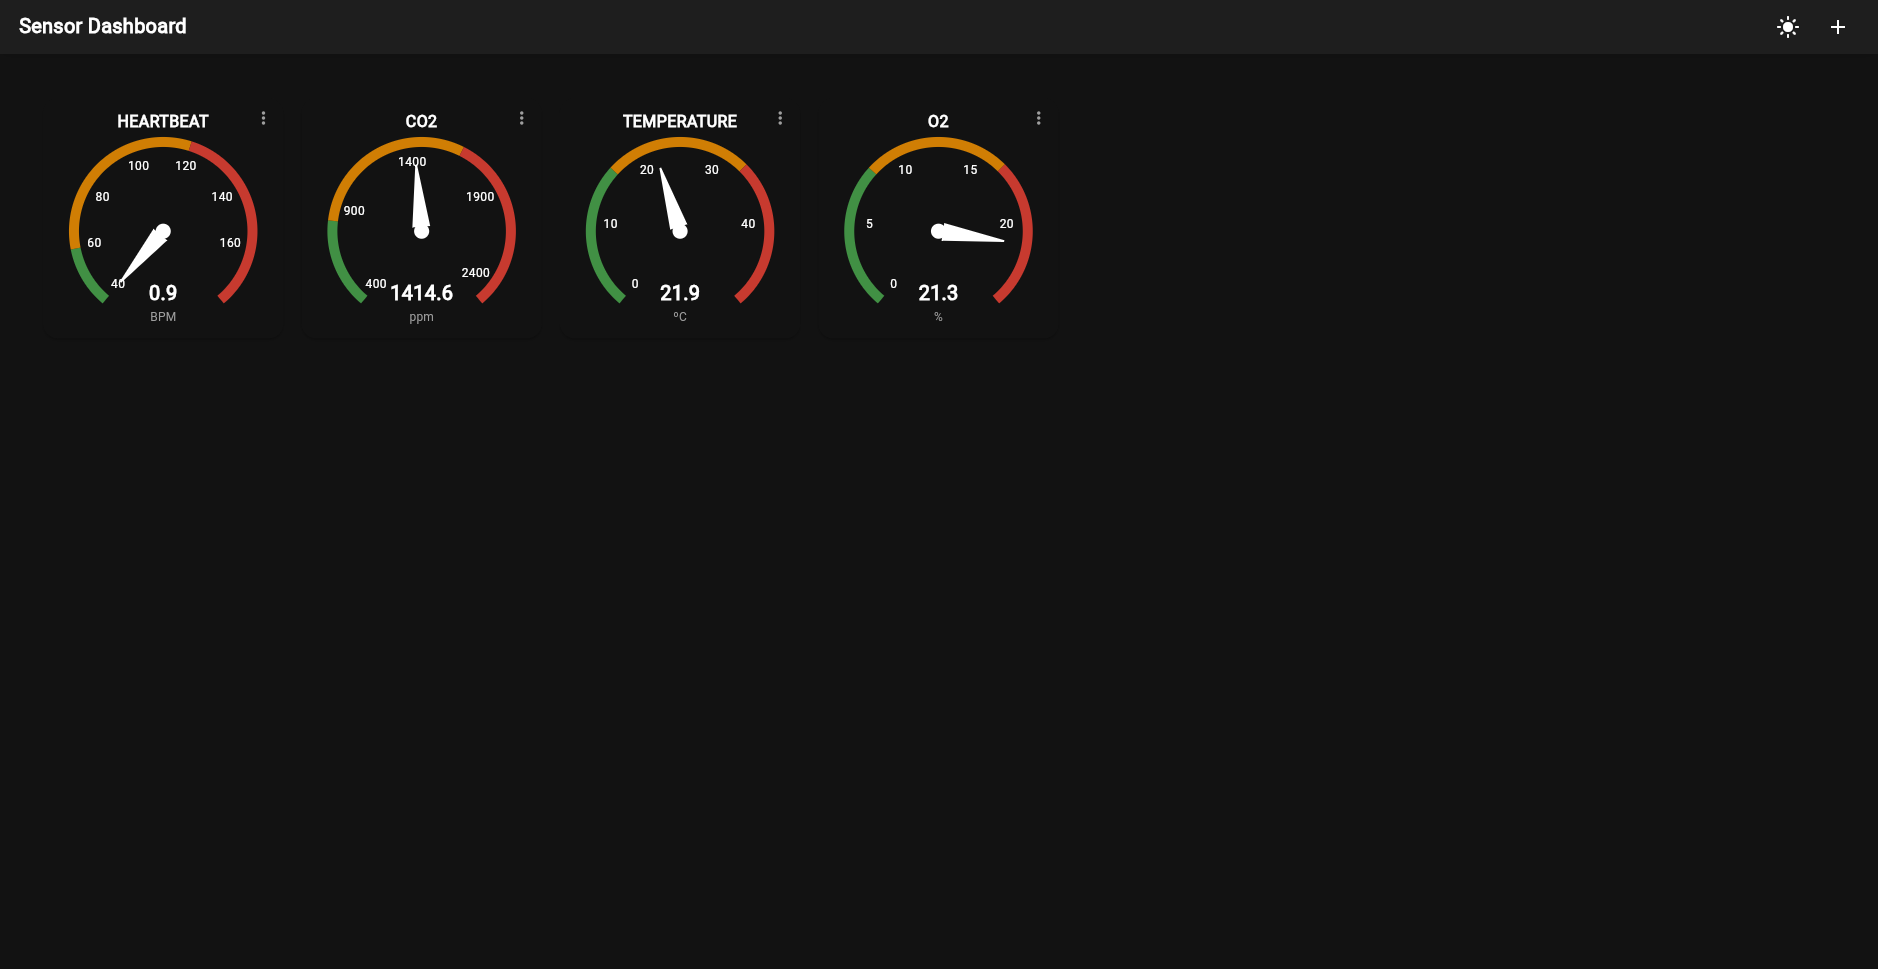
\includegraphics[width=\textwidth]{imagens/web_initial_screen.png}
		\caption{Interface Web}
		\label{subfig:web_intial_screen}
	\end{subfigure}
	\hfill
	\begin{subfigure}{0.30\linewidth}
		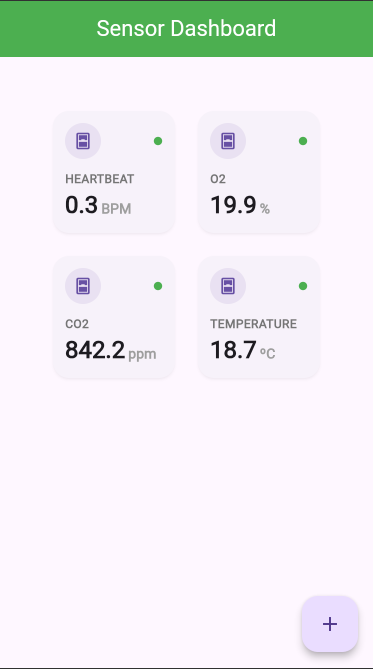
\includegraphics[width=\textwidth]{imagens/mobile_initial_screen.png}
		\caption{Interface Mobile}
		\label{subfig:mobile_intial_screen}
	\end{subfigure}
	
	\caption{Ecrã inicial com as medições dos sensores em tempo real.}
	\label{fig:initial_screen}
\end{figure}

\subsection{Ecrã para inserção de novos sensores}
Para adicionar novos sensores ao painel principal, o utilizador acede a um menu de seleção. Ao abrir essa interface, a aplicação executa uma \textit{Query} GraphQL ao \textit{back-end} para obter a lista atualizada de todos os nós e sensores registados na base de dados.

Devido às diferenças de navegação entre plataformas, na versão \textit{Mobile} (Figura \ref{subfig:mobile_add_sensor_screen}) esta funcionalidade é apresentada num ecrã dedicado, para haver uma área de toque maior. Por outro lado, na versão \textit{Web} (Figura \ref{subfig:web_add_sensor_screen}), a lista é apresentada sob a forma de uma janela sobreposta (\textit{Dialog}). Ao guardar a seleção, as escolhas são persistidas localmente no dispositivo e as respetivas \textit{subscriptions} de tempo real são ativadas no ecrã inicial.

\begin{figure}[h]
	\centering
	\begin{subfigure}{0.65\linewidth}
		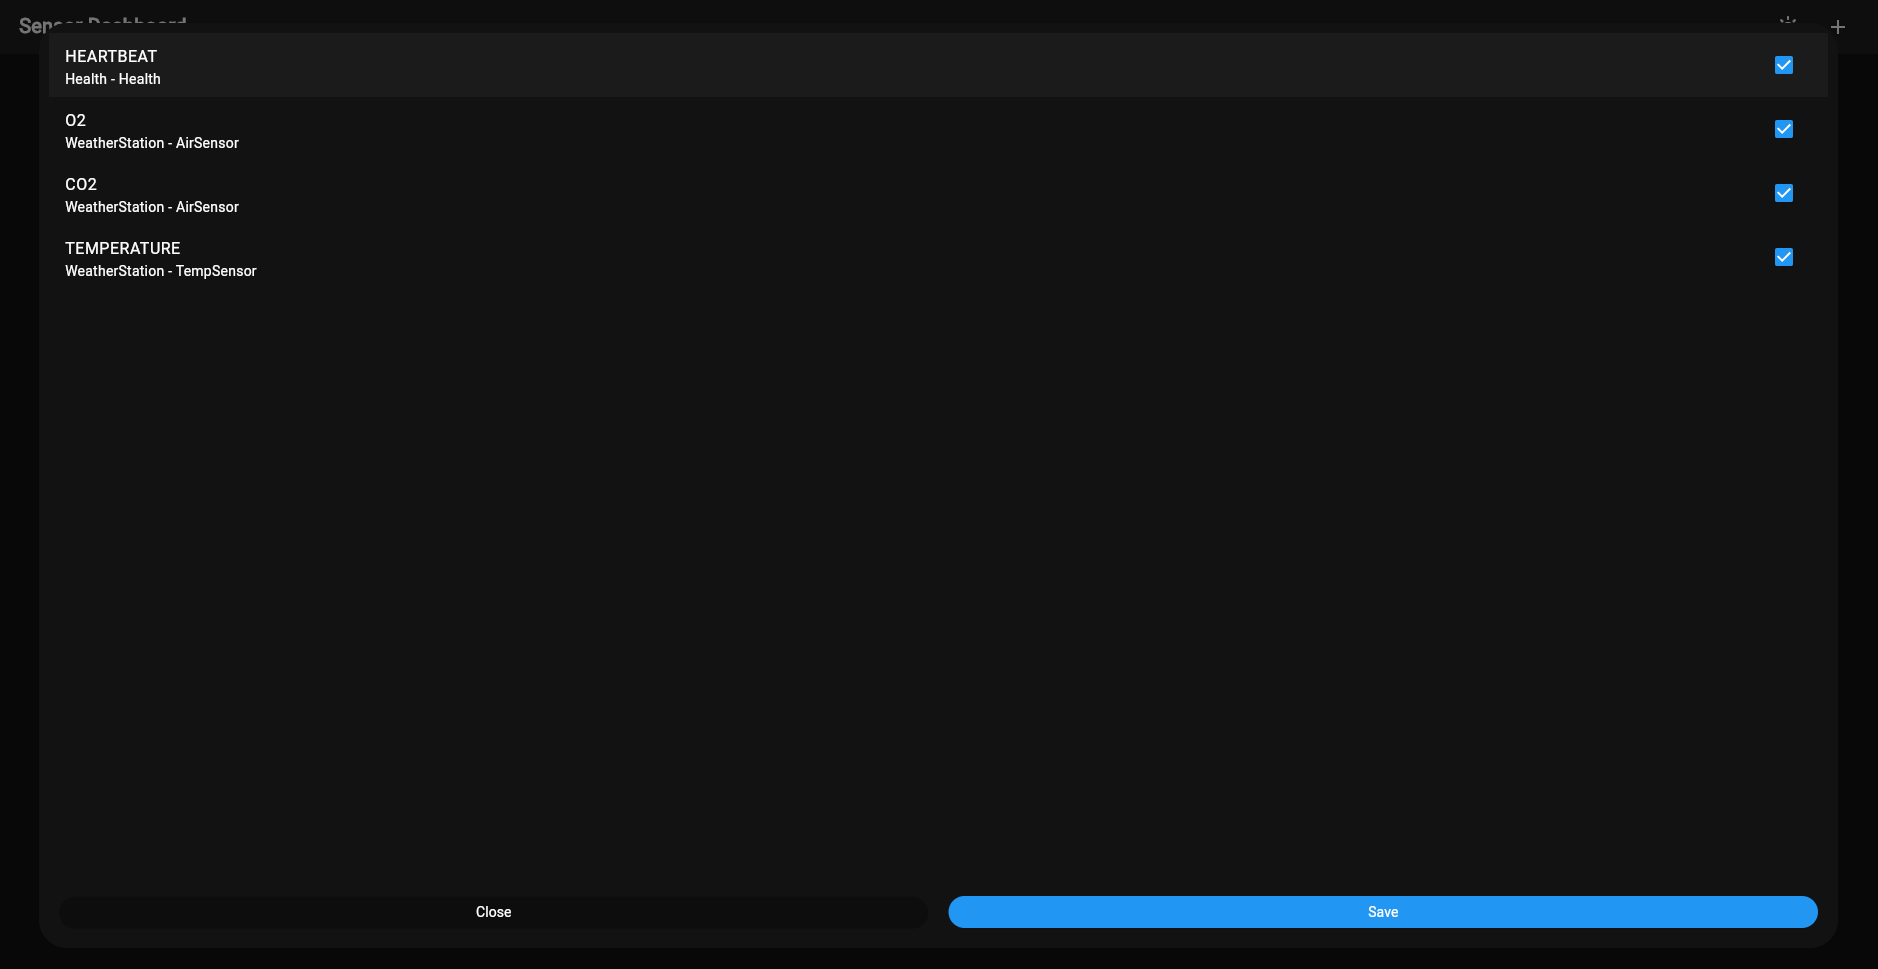
\includegraphics[width=\textwidth]{imagens/web_add_sensor_screen.png}
		\caption{Interface Web}
		\label{subfig:web_add_sensor_screen}
	\end{subfigure}
	\hfill
	\begin{subfigure}{0.30\linewidth}
		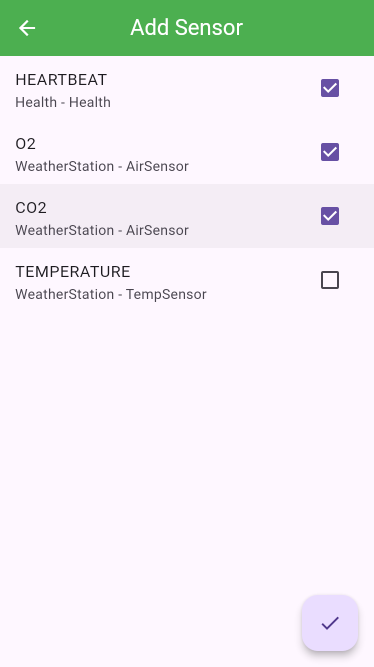
\includegraphics[width=\textwidth]{imagens/mobile_add_sensor_screen.png}
		\caption{Interface Mobile}
		\label{subfig:mobile_add_sensor_screen}
	\end{subfigure}
	
	\caption{Interface para adição e gestão de sensores no painel.}
	\label{fig:add_sensor_screen}
\end{figure}

\subsection{Gráfico histórico de medições}
A análise temporal dos dados é crucial para identificar tendências e anomalias. Ao selecionar um sensor específico, o utilizador tem acesso a um gráfico de linhas que ilustra o histórico recente de medições.

No gráfico, a integração com o servidor ocorre em duas fases simultâneas: primeiro, uma \textit{Query} GraphQL é realizada para carregar o histórico de dados guardados na base de dados, de modo a desenhar a linha inicial; de seguida, os dados provenientes da \textit{subscription} em tempo real são injetados diretamente no gráfico, fazendo com que a linha avance dinamicamente. Na versão \textit{Web} (Figura \ref{subfig:web_data_temporal_chart}), este gráfico é exibido através de um painel lateral (\textit{Side Panel}). Na aplicação \textit{Mobile} (Figura \ref{subfig:mobile_data_temporal_chart}), devido às limitações físicas do ecrã, o gráfico é exibido num novo ecrã.

\begin{figure}[h]
	\centering
	\begin{subfigure}{0.65\linewidth}
		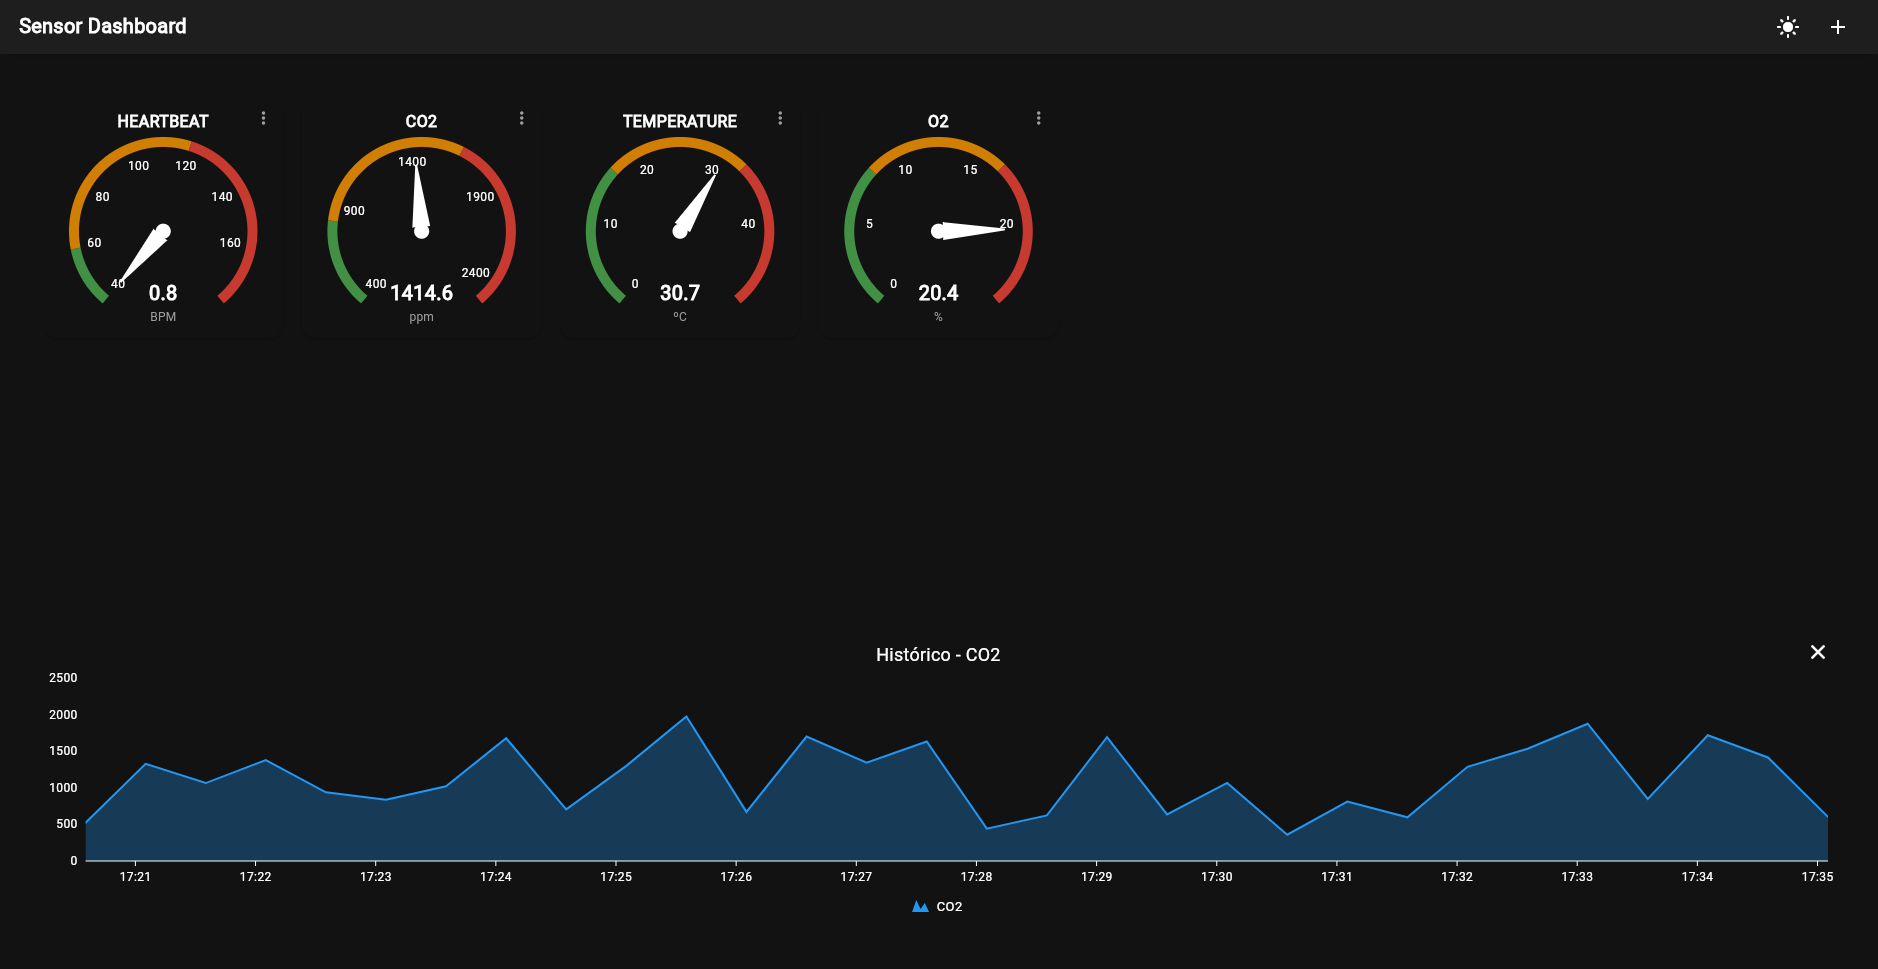
\includegraphics[width=\textwidth]{imagens/web_data_temporal_chart.png}
		\caption{Interface Web}
		\label{subfig:web_data_temporal_chart}
	\end{subfigure}
	\hfill
	\begin{subfigure}{0.30\linewidth}
		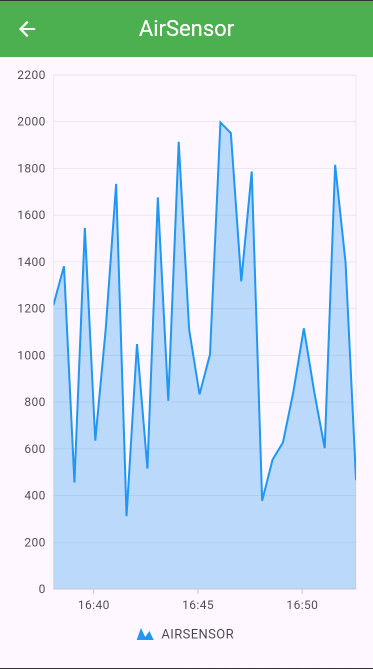
\includegraphics[width=\textwidth]{imagens/mobile_data_temporal_chart.png}
		\caption{Interface Mobile}
		\label{subfig:mobile_data_temporal_chart}
	\end{subfigure}
	
	\caption{Gráfico com o histórico temporal de medições de um sensor selecionado.}
	\label{fig:data_temporal_chart}
\end{figure}

\subsection{Alterar mínimos e máximos}

Como referido na Secção \ref{subsec:ecra_inicial}, o \textit{dashboard} \textit{Web} utiliza gráficos radiais (\textit{Gauges}), que necessitam de limites pré-definidos para contextualizar adequadamente se as medições estão dentro de um intervalo admissível.

Embora os sensores recebam valores genéricos ao serem adicionados, o utilizador pode ajustá-los através de uma janela sobreposta (\textit{Dialog}), acessível no canto superior direito de cada mostrador (Figura \ref{fig:web_change_min_max}). Esta parametrização ajusta dinamicamente a escala do gráfico, permitindo focar a monitorização num intervalo de valores mais exato.

Adicionalmente, este painel permite a remoção rápida do sensor. Todas as alterações efetuadas são guardadas de forma persistente através das preferências locais (\textit{SharedPreferences}), assegurando que as configurações visuais não se perdem ao reiniciar a aplicação.

\begin{figure}[h]
	\centering
	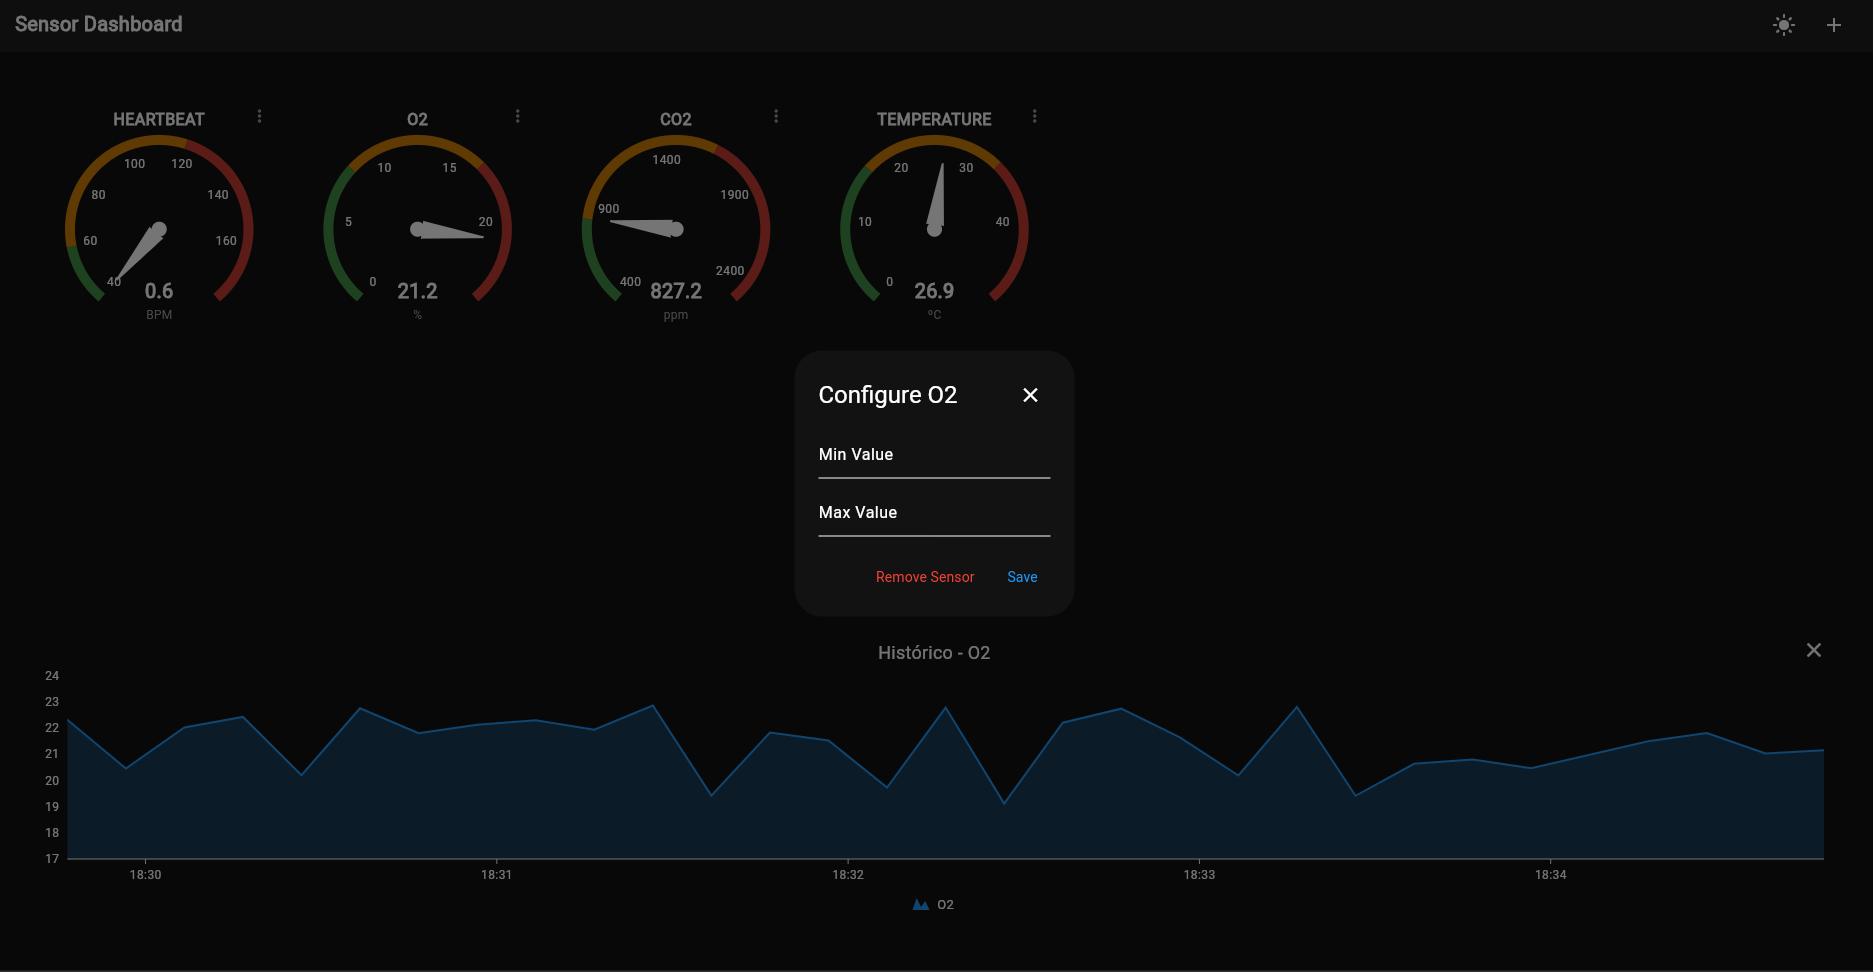
\includegraphics[width=0.7\linewidth]{imagens/web_change_min_max}
	\caption{Dialog para edição dos limites do mostrador e remoção do sensor.}
	\label{fig:web_change_min_max}
\end{figure}


\section{Metodologia de Avaliação e Desempenho Individual} \label{sec:desempenho_individual}

A atribuição de responsabilidades no decorrer deste projeto ocorreu de forma orgânica. Após uma fase inicial de investigação e exploração das tecnologias adotadas, a divisão de tarefas consolidou-se naturalmente: o desenvolvimento da aplicação cliente (\textit{front-end}), que ficou a cargo do Hugo, e a arquitetura e desenvolvimento do servidor (\textit{back-end}), assumida pelo Diogo. 

\subsection{Critérios de Atribuição de \textit{Story Points}}
A atribuição de \textit{Story Points} foi realizada com base na escala de Fibonacci. Esta métrica avaliou a complexidade técnica, o número de operações envolvidas e as integrações necessárias de cada tarefa de desenvolvimento:
\begin{itemize}
	\item \textbf{1 a 3 pontos (Complexidade Baixa a Média-Baixa):} Tarefas com requisitos bem definidos, configurações base (como a injeção de dependências ou estrutura inicial da aplicação), definição da API GraphQL ou parametrizações simples na interface gráfica (como definir limites para os gráficos radiais).
	\item \textbf{5 pontos (Complexidade Média):} Tarefas com integrações entre múltiplos componentes do sistema, construção do \textit{Dashboard} interativo ou configuração das pontes MQTT e GraphQL \textit{Subscriptions}.
	\item \textbf{8 pontos (Complexidade Alta):} Tarefas tecnicamente desafiantes, exigindo manipulação assíncrona de eventos, orquestração contínua do simulador de dados e renderização de séries temporais reativas combinadas com histórico.
\end{itemize}

\subsection{Distribuição do Esforço e Contribuição}
Após a atribuição e somatório dos \textit{Story Points} (SP) de todas as fases do projeto, apurou-se um total de 68 SP. A Figura \ref{fig:distribuicao_sp} ilustra a distribuição global do esforço:

\begin{figure}[h]
	\centering
	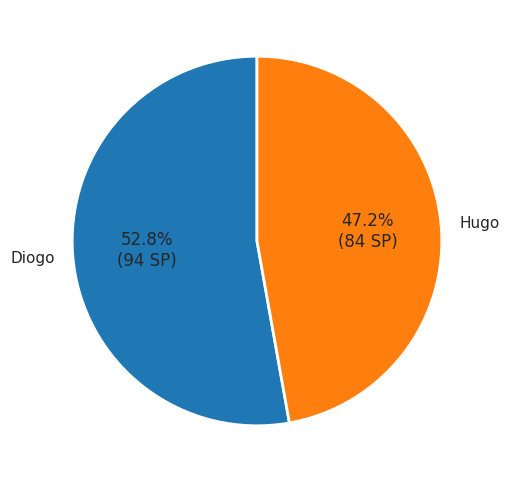
\includegraphics[width=0.5\textwidth]{imagens/desempenho_individual_story_points.png} 
	\caption{Distribuição da carga de trabalho do projeto com base em \textit{Story Points}.}
	\label{fig:distribuicao_sp}
\end{figure}

\subsubsection{Contribuição: Diogo (52.8\% -- 94 SP)}
O Diogo assumiu a responsabilidade pela arquitetura e desenvolvimento do \textit{back-end} em \textit{Scala} utilizando o ecossistema \textit{ZIO}. A sua carga de trabalho esteve concentrada no processamento não-bloqueante de dados e na infraestrutura reativa:
\begin{itemize}
	\item \textbf{Simulador e Integração MQTT:} A tarefa mais exigente do \textit{back-end} (avaliada em 8 SP), que envolveu a integração e orquestração do simulador de sensores IoT, garantindo o correto fluxo de dados em formato \textit{Sparkplug B} através do \textit{broker} MQTT.
	\item \textbf{Processamento de Eventos:} Tarefas de média-alta complexidade relativas ao processamento em memória do estado dos nós (\textit{Nodes}) e telemetrias (\textit{Metrics}), recorrendo à programação orientada a eventos.
	\item \textbf{Motor GraphQL e Base de Dados:} Configuração da infraestrutura persistente (\textit{PostgreSQL}) e implementação da API GraphQL (com recurso à biblioteca \textit{Caliban}), culminando na gestão das \textit{subscriptions} reativas.
\end{itemize}

\subsubsection{Contribuição: Hugo (47.2\% -- 84 SP)}
O Hugo assumiu a estruturação, lógica e interface visual do cliente interativo (\textit{front-end}) em \textit{Flutter}. A sua contribuição focou-se no domínio de apresentação reativa, sincronização de estado (\textit{MVVM}) e componentes visuais de análise:
\begin{itemize}
	\item \textbf{Gráficos e Séries Temporais:} A tarefa de maior exigência técnica no cliente, que consistiu em fundir dados históricos com eventos em tempo real provenientes das \textit{subscriptions}, traduzindo-os em gráficos de linhas dinâmicos (\textit{Time Series Charts}).
	\item \textbf{Sincronismo em Tempo Real:} Configuração complexa do cliente GraphQL no lado da aplicação móvel/web, gerindo as sessões \textit{WebSocket} para a atualização contínua de dados.
	\item \textbf{Dashboard Visual:} O desenvolvimento do ecrã de controlo, que incluiu a renderização dos mostradores radiais (\textit{Gauges}), permitindo ainda configurações locais personalizadas de limites mínimos e máximos.
\end{itemize}


\section{Conclusão} \label{sec:conclusao}

O presente relatório documenta a criação de um sistema reativo para monitorização de sensores IoT, destacando-se pela separação de responsabilidades entre o \textit{back-end} e o \textit{front-end}.

No \textit{back-end}, desenvolvido em \textit{Scala} com o ecossistema \textit{ZIO}, implementou-se uma arquitetura não bloqueante orientada a eventos (\textit{Event-Driven}), integrada com um \textit{broker} MQTT (\textit{Sparkplug B}). Simultaneamente, a Programação Orientada a Aspetos (AOP) que permitiu isolar o registo de métricas (\textit{logging}), mantendo a lógica de negócio modular.

No \textit{front-end}, o \textit{Flutter} permitiu gerar interfaces \textit{Web} e \textit{Mobile} a partir de uma base de código única. A conjugação do padrão MVVM com \textit{subscriptions GraphQL} (\textit{WebSockets}) assegurou um fluxo de comunicação eficiente, refletindo as leituras dos sensores nos mostradores gráficos em tempo real e com latência impercetível.

\subsection{Trabalho Futuro}
Embora os requisitos propostos para o sistema tenham sido plenamente cumpridos, o ciclo de desenvolvimento de \textit{software} é iterativo. Dessa forma, identificam-se as seguintes melhorias potenciais para a evolução contínua da plataforma:

\begin{itemize}
	\item \textbf{Sistema de Alertas e Notificações:} Aproveitar os limites mínimos e máximos já definidos no \textit{front-end} para criar um mecanismo de atuação no servidor, capaz de disparar notificações \textit{push} ou alertas por email sempre que um sensor registe valores anómalos.
	
	\item \textbf{Segurança e Autenticação:} Integrar um sistema de autenticação e autorização (como JWT ou \textit{OAuth}) para garantir que apenas operadores credenciados têm acesso ao painel de monitorização e à \textit{API GraphQL}.
\end{itemize}

\end{document}
